\documentclass{beamer}
\usetheme{Goettingen}
% \usecolortheme{beaver}
% \usebackgroundtemplate{\includegraphics[width=\paperwidth,height=\paperheight]{background.jpg}}
\usepackage{tikz}
\usepackage{pgfplots}
\usepackage{pgfplotstable}
\usepackage{graphicx}
\usepackage[brazil]{babel}
\usepackage{hyperref}
% \usepackage{subcaption}
% \usepackage{amsmath}

\newcommand{\femboy}{\textit{Femboy}}
\newcommand{\femboys}{\textit{Femboys}}
\newcommand{\addNewlines}[1]{\vspace*{#1\baselineskip}}


\title{Por que \femboys{} são o pilar da sociedade?}
\author{Uma apresentação por: \vscpace
Rodrigo Aroeira}
\date{27 de abril de 2024}

\pgfplotsset{compat=1.18}

\begin{document}
\maketitle


\begin{frame}{\begin{center}
    \Large{O que é um \femboy?}
\end{center}}

\begin{figure}
    % \centering
    
\includegraphics[width=0.3\textwidth]{femboy.jpg}
    \caption{Um exemplo de \femboy}
\end{figure}

\end{frame}

\begin{frame}{}
   \begin{enumerate}
    \item Origem do Termo
    \item Por que existem?
    \item Impacto na Sociedade
   \end{enumerate} 
\end{frame}

% MARK: - Origem do Termo

\begin{frame}{1 - Origem do Termo}
\begin{center}
    \Huge{Etimologia}
    \addNewlines{3}
\end{center}

\begin{itemize}
    \item Origem nos anos 90
    \item Abreviação de \textit{fem} (abreviação de \textit{feminine} ou \textit{femme}) + \textit{boy}
\end{itemize}

\end{frame}

% MARK: - Por que existem?

\begin{frame}{2 - Por que existem?}
   \begin{figure}
         \centering
         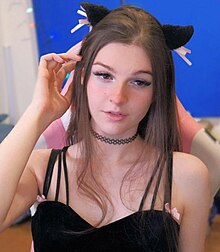
\includegraphics[width=0.5\textwidth]{finn.jpg}
         \caption{Streamer F1NN5TER}
   \end{figure} 
\end{frame}

\begin{frame}{3 - Impacto na Sociedade}
    \begin{itemize}
        \item Aumento da diversidade
        \item Quebra de estereótipos
        \item Aumento da auto-aceitação
    \end{itemize}
    
\end{frame}


\begin{frame}{Fontes}
    \url{https://en.wikipedia.org/wiki/Femboy}
    


    \url{https://www.reddit.com/r/teenagers/comments/166diso/why_do_people_become_femboys/}
\end{frame}

\end{document}